The convolution operator is defined on two functions $f(\mathbf{x})$ and $g(\mathbf{x})$, with $\mathbf{x} \in \mathbb{R}^{d}$: 

\begin{equation}
    (f * g)(\mathbf{x})=\iint_{\boldsymbol{\tau} \in \mathbb{R}^{d}} f(\boldsymbol{\tau}) g(\mathbf{x}+\boldsymbol{\tau}) d \boldsymbol{\tau}
\end{equation}

In images the function $g(\mathbf{x})$ is a 2D function, and because images are made up by a discrete and fixed grid of pixel we can see turn the integrals in the discrete sum of product between $f$ and $g$.

Such a regular structure is not intrinsic of point clouds, and thus convolution is not easily implementable.

To tackle this problem without using an intermediate representation of the point cloud (as seen with projection based approaches) specialized convolution operators have been proposed.

\paragraph{PointConv}
In this section we will explore the PointConv operation, proposed by Wenxuan Wu et al. \cite{PointConv}

A point cloud is a set of 3D points $(x,y,z)$, so the 3D convolution can be written as: 

\begin{equation}
    \begin{array}{l}
\operatorname{Conv}(W, F)_{x y z}= 
\quad \iiint_{\left(\delta_{x}, \delta_{y}, \delta_{z}\right) \in G} W\left(\delta_{x}, \delta_{y}, \delta_{z}\right) F\left(x+\delta_{x}, y+\delta_{y}, z+\delta_{z}\right) d \delta_{x} \delta_{y} \delta_{z}
\end{array}
\end{equation}

where $W(\delta_{x}, \delta_{y}, \delta_{z})$ is the weight function and $F\left(x+\delta_{x}, y+\delta_{y}, z+\delta_{z}\right)$ is the feature of a point in the local region $G$ centered in  $p = (x,y,z)$.

Point clouds, unlike images, are not uniformly sampled from the 3D space: the points $(\delta_{x}, \delta_{y}, \delta_{z})$ do not have a fixed structure in the local region: there could be subregions with more dense sampling and subregions with more sparse points, thus transforming the integral into a discrete sum is not trivial.
To deal with uneven sampling the authors introduced the inverse sparsity function $S(x,y,z)$. The PointConv operator is thus defined as:

\begin{equation}
    \operatorname{PointConv} (S, W, F)_{x y z}=
\sum_{\left(\delta_{x}, \delta_{y}, \delta_{z}\right) \in G} S\left(\delta_{x}, \delta_{y}, \delta_{z}\right) W\left(\delta_{x}, \delta_{y}, \delta_{z}\right) F\left(x+\delta_{x}, y+\delta_{y}, z+\delta_{z}\right)
\end{equation}

%TODO punti da trattare
\begin{itemize}
    \item The $W$ function can be approximated by a MLP.
    \item The $S$ function is calculated using a kernel density estimator.
    \item practical: feature encoding layer (sampling, grouping (che poi è la ricerca dei neighbor), pointconv)
    \item (se c'è spazio) efficient pointconv
    \item (se c'è spazio) ablation test
\end{itemize}

\begin{figure}[h]
    \centering
    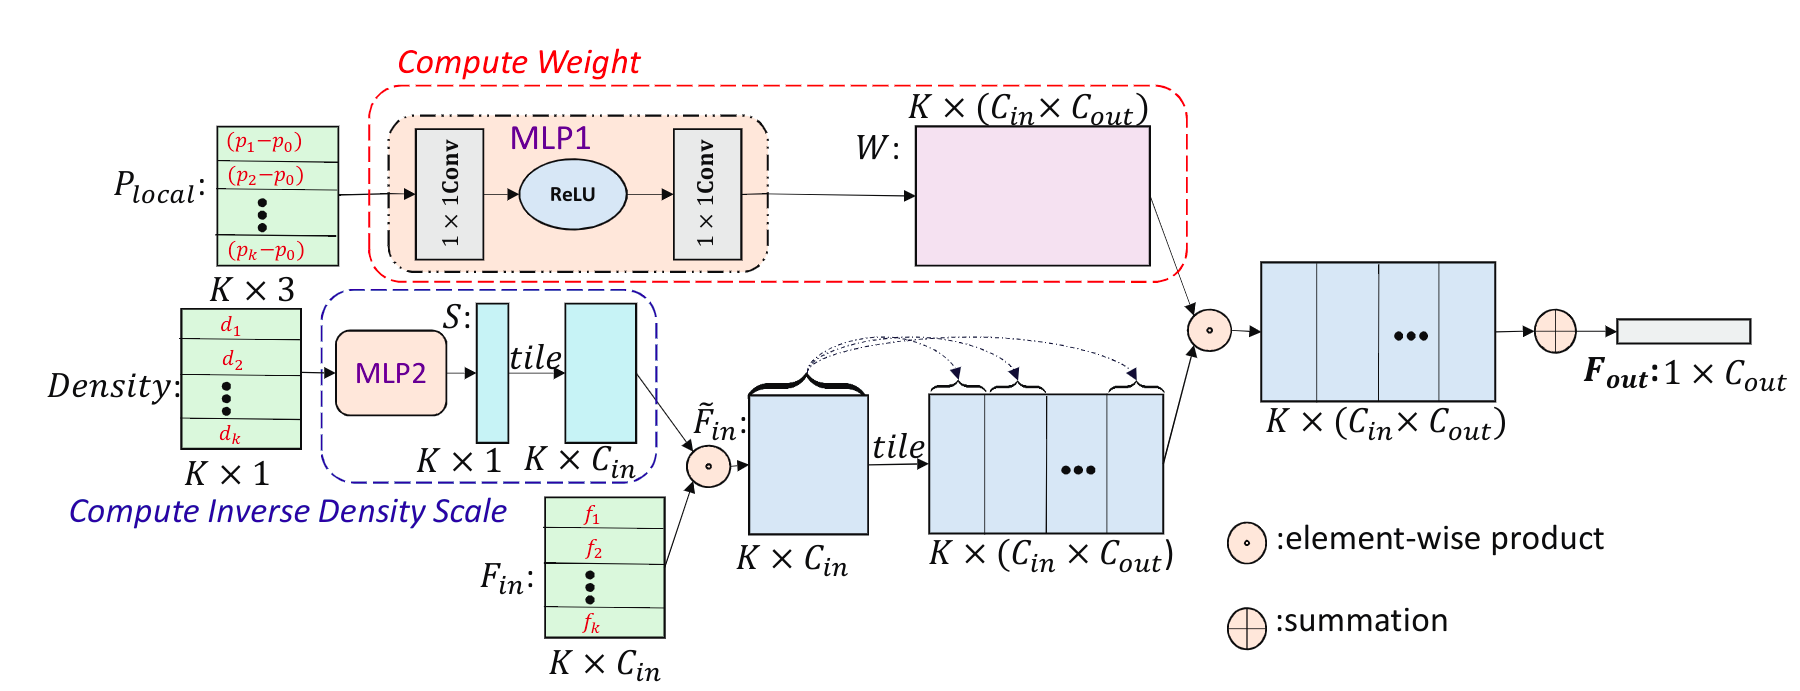
\includegraphics[width=\textwidth]{pointconv.png}
    \caption{Caption}
    \label{fig:pointconvOperator}
\end{figure}

